 \documentclass{beamer}

\usetheme{MagdeburgFIN}
\usefonttheme{structurebold}
\usepackage{graphicx}
\usepackage{float}
\usepackage{url}
\usepackage{pdfpages}
\usepackage[ngerman]{babel}
\usepackage[utf8]{inputenc}

\title{Thread Pool in GeckoDB/BOLSTER}
\subtitle{Milestone II: Concept \& additional literature research}
\author{Johann Wagner, Johannes Wünsche, Marten Wallewein-Eising, Robert Jenderise, Benedikt Zeilinger}
\date{\today}
\institute{Otto von Guericke University, Magdeburg}

% Milestone II: Concept & additional literature research

\begin{document}

\begin{frame}[plain]
 \titlepage
\end{frame}

\section[Agenda]{}
	\begin{frame}
	\frametitle{Agenda}
	\tableofcontents
	\end{frame}

\section{Previously...}
\begin{frame}
	\frametitle{Previously in Thread Pool in GeckoDB/BOLSTER}
	\begin{itemize}
		\item Operations are spawning dozens of threads, which are not handled and managed
		\item Heavy overhead of creating and removing threads
		\item After some operations profiler dies (too many threads)
		\item Because of Late/Early Materialization and Prefetching Support, existing libs are not adequate
	\end{itemize}
	\begin{center}
		
\includegraphics[width=0.3\textwidth]{img/thumbs_down.png}
	\end{center}
\end{frame}

\begin{frame}
	\frametitle{Previously in Thread Pool in GeckoDB/BOLSTER}
	\begin{itemize}
		\item Reuse of Threads with thread pools.
		\item Reduce overhead of thread management
		\item Improve maintainability of parallel code
		\item Support the performance and design requirements (e.g. Future and Promise) of BOLSTER
	\end{itemize}
	\begin{center}
		
\includegraphics[width=0.3\textwidth]{img/thumbs_up.png}
	\end{center}
\end{frame}

\section{Concept and Design}
\begin{frame}
	\frametitle{Concept}
	\begin{itemize}
		\item Thread pool with runtime dynamic amount of threads and priority queue
		\item Tasks are not preemtable and independent
		\item Array of tasks passed to an enqueue function, which waits until all tasks are finished
		\item Threads without tasks idle until they get a new one
		\item Monitoring/managing state and assigned task of each thread
		\item Allow usage of multiple, independent thread pool instances 
	\end{itemize}
\end{frame}

\begin{frame}
\frametitle{Design}
	\begin{center}
		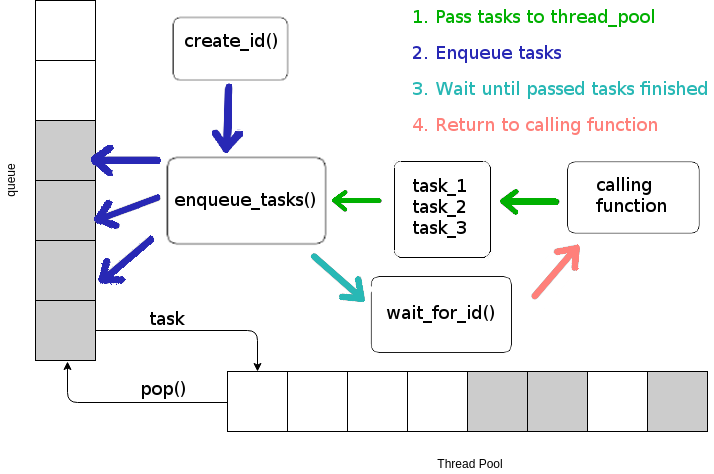
\includegraphics[width=0.9\textwidth]{img/pool_queue.png}
	\end{center}
\end{frame}

\section{Current Progress}
\begin{frame}
	\frametitle{Current Progress}
	We...
	\begin{itemize}
		\item Implemented the priority queue 
		\item Implemented the creation of threads and the assigning of tasks
		\item Added gtest framework to project and wrote tests for pool and queue
		\item Began first implementations of waiting for tasks to be finished
		\item Measure performance of task assigning and execution
	\end{itemize}
\end{frame}

\section{Next Steps}
\begin{frame}
	\frametitle{Next Steps}
	We have to ...
	\begin{itemize}
		\item Find an efficient way to wait for tasks
		\item Find an efficient way to idle threads until they get the next tasks
		\item Add metrics to threads and tasks and measure performance and overhead
		\item Add tests for all implementations
	\end{itemize}
\end{frame}

\begin{frame}
	\frametitle{Next Steps - Scheduling}
	Current approach:  
	\begin{itemize}
		\item Threads ask for next task in queue
	\end{itemize}
	Desired implementation: 
	\begin{itemize}
		\item Make own scheduling, assign tasks to threads
		\item Add possibility to try different scheduling approaches
		\item Measure thread idle and busy time for the approaches
	\end{itemize}
\end{frame}

\section{Additional Literature Research}
    \begin{frame}
        \frametitle{Additional Literature Research}
        \begin{itemize}
            \item Albahari, Joseph. \emph{Threading in C.} online. Joseph Albahari \& O’Reilly Media, Inc (2006).
            \item Rasmussen, Rasmus V., and Michael A. Trick. \emph{Round robin scheduling–a survey.} European Journal of Operational Research 188.3 (2008): 617-636.
            \item Shreedhar, Madhavapeddi, and George Varghese. \emph{Efficient fair queueing using deficit round robin.} ACM SIGCOMM Computer Communication Review. Vol. 25. No. 4. ACM, 1995.
        \end{itemize}
    \end{frame}



    \begin{frame}
        \frametitle{Thank you for your attention!}
    \end{frame}
\end{document}
